\documentclass[notitlepage,a4paper,twoside,10pt]{article}


\usepackage{ngerman} 
\usepackage[latin1]{inputenc} 
\usepackage[T1]{fontenc} 
\usepackage[pdftex]{graphicx} 
\usepackage[pdftex,bookmarks=true,colorlinks,linkcolor=blue,urlcolor=blue,citecolor=blue]{hyperref}

\sloppy

%opening
\title{Daten verschl�sseln mit TrueCrypt}
\author{mit TrueCrypt f�r WINDOWS}
\date{\today}

\hypersetup {
    pdftitle= { Daten verschl�sseln mit TrueCrypt f�r WINDOWS}
    pdfkeywords= {Daten verschl�sseln Verschl�selung TrueCrypt WINDOWS }
}


\begin{document}
\maketitle
\tableofcontents

\section{Einleitung}
Dass die Verschl�sselung von Daten der Erhaltung einer Privatsph�re dient, bemerkt man sp�testens, wenn ein USB-Stick verloren geht. Wird ein Laptop gestohlen, m�chte man die Fotosammlung sicher nicht im Internet sehen.\\

Investigative Journalisten, Rechtsanw�lte und auch Priester haben das Recht und die Pflicht, ihre Informanten bzw. Klienten zu sch�tzen. Sie sollten sich fr�hzeitig Gedanken �ber ein Konzept zur Verschl�sselung machen. Es ist wirklich �rgerlich, wenn die Rote Hilfe einen unverschl�sselten Datentr�ger mit Mitgliederdaten verliert. Das kann ernste Konsequenzen haben.\\

Als Whistleblower sind besondere Anforderungen an die Datensicherheit zu stellen. Neben der sicheren Aufbewahrung kommt es auch darauf an, keine Spuren auf den Rechnern zu hinterlassen. Im Fall Bradley Mannings konnten Forensiker viele Daten wieder herstellen

Die kurzen Beispiele zeigen, dass unterschiedliche Anforderungen an eine Verschl�sselung bestehen k�nnen. Bevor man wild anf�ngt, alles irgendwie zu verschl�sseln, sollte man sich Gedanken �ber die Bedrohung machen, gegen die man sich sch�tzen will:
\begin{enumerate}
 \item \textbf{Schutz sensibler Daten} wie z.B. Passwortlisten, Revocation Certificates o.�. erfordert die Speicherung in einem Container oder verschl�sselten Archiv, welches auch im normalen Betrieb geschlossen ist.
\item \textbf{Schutz aller pers�nlichen Daten} bei Verlust oder Diebstahl von Laptop oder USB-Stick erfordert eine Software, die transparent arbeitet ohne den Nutzer zu behindern und bei korrekter Anmeldung m�glichst automatisch den Daten-Container �ffnet (beispielsweise TrueCrypt f�r WINDOWS oder DM-Crypt f�r Linux). 
\item \textbf{Backups auf externen Medien} enthalten in der Regel die wichtigen privaten Daten und sollten ebenfalls verschl�sselt sein. Dabei sollte die Wiederherstellung auch bei totalem Datenverlust m�glich sein. Es ist nicht sinnvoll, die Daten mit einem PGP-Schl�ssel zu chiffrieren, der nach einem Crash nicht mehr verf�gbar ist.
\item Wer eine \textbf{Manipulation der Sytemdaten} bef�rchtet, kann seinen Rechner komplett verschl�sseln (mit Truecrypt f�r WINDOWS, DM-Crypt f�r Linux oder GELI f�r FreeBSD).\\
\end{enumerate}

Zur \textbf{Herausgabe von Schl�sseln} im Fall einer Beschlagnahme des Rechners oder verschl�sselten Datentr�gers gibt es immer wieder Missverst�ndnisse.\\

In Deutschland gelten folgende gesetzlichen Reglungen:
\begin{itemize}
 \item Richten sich die Ermittlungen gegen den Besitzer des Rechners oder Datentr�gers muss man grunds�tzlich keine Keys herausgeben.
\item Richten sich die Ermittlungen gegen Dritte, kann man die Herausgabe von Keys verweigern, wenn man sich auf das Recht zur Zeugnisverweigerung berufen oder glaubhaft(!) versichern kann, dass man sich damit selbst belasten w�rde. Im Zweifel sollte man einen Anwalt konsultieren.
\end{itemize}

In Gro�britannien ist es bereits anders. Gem�� dem dort seit Oktober 2007 geltendem RIPA-Act k�nnen Nutzer von Verschl�sselung unter Strafandrohung zur Herausgabe der Schl�ssel gezwungen werden. Es drohen bis zu 2 Jahre Gef�ngnis oder Geldstrafen. Das die Anwendung des Gesetzes nicht auf die b�sen Terroristen beschr�nkt ist, kann man bei Heise.de nachlesen. Es wurde als ersten gegen eine Gruppe von Tiersch�tzern angewendet.\footnote{ \href{http://www.heise.de/newsticker/meldung/99313}{http://www.heise.de/newsticker/meldung/99313}}\\

Bei Einreise in die USA sind die Grenzbeh�rden berechtigt, elektronische Ger�te (Laptops und Smartphones) zu durchsuchen. Eine Herausgabe von Passw�rtern kann ohne Durchsuchungs�beschluss nicht erzwungen werden, aber die Beh�rden k�nnen das Ger�t aber zur weiteren Untersuchung einziehen, wenn man das Passwort nicht heraus geben will. Die EFF.org r�t, mit einer leeren, unverschl�sselten Festplatte einzureisen und ein datenloses Handy zu nutzen: \href{https://www.eff.org/wp/defending-privacy-us-border-guide-travelers-carrying-digital-devices}{https://www.eff.org/wp/defending-privacy-us-border-guide-travelers-carrying-digital-devices}

\subsubsection*{Das Container-Konzept}
Der Container ist eine passende Metapher f�r das Konzept der vorgestellten Tools \textit{Truecrypt} und \textit{DM-Crypt}. Ein Container steht rum und nimmt Platz weg, egal ob er leer oder voll ist. In diesem Fall belegt der Container Platz auf der Festplatte oder dem USB-Stick.\\

Ist der Container verschlossen, kommt niemand an die dort lagernden Daten heran. Mit einem Schl�ssel kann der Container ge�ffnet werden (gemounted: in das Dateisystem eingef�gt) und jeder, der an einem offenen Container vorbeikommt, hat Zugriff auf die dort lagernden Daten. Als Schl�ssel dient eine Passphrase und/oder Schl�sseldatei(en).\\

Der Zugriff auf Dateien innerhalb des ge�ffneten Containers erfolgt mit den Standardfunktionen f�r das �ffnen, Schlie�en und L�schen von Dateien. Auch Verzeichnisse k�nnen angelegt bzw. gel�scht werden. Die Verschl�sselung erfolgt transparent ohne weiteres Zutun des Nutzers.\\

Ein Container sch�tzt die Daten nur, wenn er geschlossen ist! Wenn man keinen ZUgriff auf die Daten braucht, sollte man den Container schlie�en. Einerseits ist bei einem ge�ffneten Container ein direkter Zugriff auf die Daten m�glich. Au�erdem k�nnen bei einem ge�ffneten Container die kryptografischen Schl�ssel aus dem RAM des Rechners ausgelesen und sp�ter zum Entschl�sseln der Daten genutzt werden. Elcomsoft bietet mit dem \textit{Forensic Disk Decryptor} eine Tool f�r diesen Angriff auf Truecrypt, PGP und Bitlocker.\footnote{ \href{http://www.elcomsoft.com/news/531.html}{http://www.elcomsoft.com/news/531.html}}
\newpage
\section{Truecrypt f�r WINDOWS}
Truecrypt basiert auf dem Projekt \textit{Encryption for the masses}. Die Software bietet transparente Ver- und Entschl�sselung beim Laden oder Speichern von Daten unter WINDOWS XP/2000/2003 und Linux. Neben der Verschl�sselung von Daten auf der Festplatte ist es auch f�r USB-Sticks geeignet.\\

Eine passende Metapher f�r das Konzept von Truecrypt ist der Container. Ein Container steht rum und nimmt Platz weg, egal ob er leer oder voll ist. In diesem Fall belegt der Container Platz auf der Festplatte oder dem USB-Stick.\\

Ist der Container verschlossen, kommt niemand an die dort lagernden Daten heran. Mit einem Schl�ssel kann der Container ge�ffnet werden (gemounted: in das Dateisystem eingef�gt) und jeder, der an einem offenen Container vorbeikommt, hat Zugriff auf die dort lagernden Daten. Als Schl�ssel dient eine Passphrase und/oder Schl�sseldatei(en).\\

Der Zugriff auf Dateien innerhalb des ge�ffneten Containers erfolgt mit den Standardfunktionen f�r das �ffnen, Schlie�en und L�schen von Dateien. Auch Verzeichnisse k�nnen angelegt bzw. gel�scht werden. Die Verschl�sselung erfolgt transparent ohne weiteres Zutun des Nutzers.

\subsubsection*{Mit doppeltem Boden}
Ein Feature von Truecrypt ist das Konzept des \textit{versteckten Volumes}, eine Art doppelter Boden f�r den Container.\\

Der Zugriff auf diesen Bereich ist mit einem zweiten Schl�ssel gesch�tzt, einer weiteren Passphrase und/oder Schl�sseldatei(en). �ffnet man den Container mit dem ersten Schl�ssel, erh�lt man Zugriff auf den �u�eren Bereich. Verwendet man den zweiten Schl�ssel zum �ffnen des Containers, erh�lt man Zugriff auf den versteckten Inhalt hinter dem doppelten Boden.\\

W�hrend ein einfacher Container leicht als verschl�sselter Bereich erkennbar ist, kann der doppelte Boden innerhalb eines Containers ohne Kenntnis des zweiten Schl�ssels nicht nachgewiesen werden. Ist man zur Herausgabe der Schl�ssel gezwungen, kann man versuchen, nur den Schl�ssel f�r den �u�eren Container auszuh�ndigen und die Existenz des doppelten Bodens zu leugnen.\\

Ob es plausibel ist, die Existenz des doppelten Bodens zu leugnen, h�ngt von vielen Faktoren ab. Zeigt z.B. die Historie der g�ffneten Dokumente einer Textverarbeitung, dass vor kurzem auf einen verschl�sselten Bereich zugegriffen wurde, und man pr�sentiert einen �u�eren Container, dessen letzte �nderung Monate zur�ck liegt, trifft man wahrscheinlich auf einen ver�rgerten Richter.\\

Auch der Index verschiedener Programme f�r die Indexierung der Dokumente auf dem lokalen Rechner (WINDOWS Suche, Google Desktop Search...) liefern m�glicherweise Hinweise auf den versteckten Container.\\

Wie gulli.com am 6.10.08 berichtete, ist es unter Umst�nden m�glich, die Existens des versteckten Volumes nachzuweisen. Also Vorsicht bei Nutzung dieses Features.

\subsection{Truecrypt installieren}
F�r die Installation von Truecrypt werden folgende Pakete ben�tigt:

\begin{itemize}
 \item Truecrypt von der Site des Projektes \href{http://www.truecrypt.org}{www.truecrypt.org}
\item Deutsche Sprachanpassung aus den \href{http://www.truecrypt.org/localizations.php}{Language Packs} von Truecrypt
\end{itemize}

Nach dem Download sind die ZIP-Archive zu entpacken. In dem neuen Ordner \textit{truecrypt-x.y} findet man die Setup-Datei. Diese ist als Administrator zu starten und in dem Install-Assistenten sind die Vorgaben evtl. anzupassen.\\

Ein Klick auf den Button \textit{Install} startet den Prozess. Im Anschlu� findet man ein Icon auf dem Desktop und einen neuen Eintrag im Men�.\\

Anschlie�end ist die Datei \textit{Language.de.xml} aus dem Paket der Sprachanpassung in das Verzeichnis der installierten EXE-Datei zu kopieren.

\subsection{Gedanken zum Schl�ssel}
Bevor man einen verschl�sselten Container erstellt, sollte man sich Gedanken �ber den Schl�ssel zum �ffnen des Containers machen.
\begin{itemize}
 \item Eine \textbf{Passphrase} sollte gut merkbar sein und mindestens 20 Zeichen lang sein. Au�er Buchstaben sollte sie auch Sonderzeichen und Ziffern enthalten. Das sch�ttelt man nicht einfach aus dem �rmel. Wie w�re es mit folgender Phrase:
\begin{center}
 \texttt{das geht nur \%mich\% \_AN\_}
\end{center}
\item Ein \textbf{Keyfile} kann eine beliebige Datei mit mindestens 1024 Byte Gr��e sein. Truecrypt bietet die M�glichkeit, gute Keyfiles zu generieren (Men�punkt: \textit{Schl�sseldateien -> Schl�sseldatei aus Zufallswerten erstellen} im Hauptfenster).
\end{itemize}

Man kann z.B. einen USB-Stick mit Keyfile(s) vorbereiten. Dieser Stick enth�lt eine oder mehrere Dateien, welche als Keyfile(s) genutzt werden. Diese Datei(en) k�nnen als Standardschl�ssel definiert werden (Men�punkt: \textit{Schl�sseldateien -> Standardschl�sseldateien festlegen}). Zuk�nftig ist vor dem �ffnen eines Containers lediglich der Stick einzustecken. Es funktioniert wie ein mechanischer Schl�ssel und man wird nicht mehr mit einer Passwortabfrage bel�stigt.\\

\subsection{Verschl�sselten Container erstellen}
Startet man Truecrypt oder klickt auf das blaue Symbol im Systray, so �ffnet sich das Hauptfenster. Der Button \textit{Volume erstellen} ruft einen Assistenten auf, der schrittweise alle n�tigen Angaben zur Erstellung eines Volumes abfragt und umfangreiche Erl�uterungen bietet.\\

Eingeschr�nkte Nutzer k�nnen lediglich verschl�sselte regul�re Containerdateien erstellen.\\

Administratoren k�nnen au�erdem Festplattenpartitionen und USB-Sticks verschl�sseln, Hidden Volumes (versteckte Container) erstellen und WINDOWS komlett verschl�sseln.\\

\begin{figure}[htb]
\begin{center}
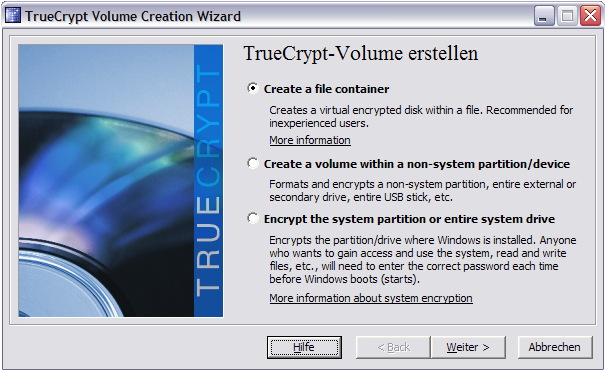
\includegraphics[scale=0.5]{../screenshots/truecrypt_1.png}
\caption{Assistent zur Erstellung eines Containers}
\label{abb:truecrypt_assi}
\end{center}
\end{figure}

Im Folgenden wird der Ablauf zur Erstellung einer verschl�sselten Containerdatei beschrieben:
\begin{enumerate}
 \item Auswahl des Containertypes (regul�res oder verstecktes Volume). Soll ein verstecktes Volume erstellt werden, ist zuerst ein normales Volume zu erstellen, in dem anschlie�end das zweite Volume versteckt werden kann.
\item Im zweiten Schritt ist der Dateiname f�r den Container anzugeben oder als Datentr�ger die Festplattenpartition bzw. der USB-Sticks (nur als Administrator). Es ist auch als eingeschr�nkter Nutzer m�glich, eine Datei auf einem USB-Stick zu erstellen. Diese Datei k�nnte 2/3 des Sticks einnehmen. Der Stick kann dann bei Notwendigkeit auch ohne Truecrypt genutzt werden.
\item Im dritten Schritt ist die Gr��e der Datei anzugeben. Dieser Schritt entf�llt, wenn eine Partition oder USB-Stick komplett verschl�sselt wird.
\item Im vierten Schritt ist der Schl�ssel f�r das �ffnen des Containers festzulegen. Ein gutes Passwort sollte mindestens 20 Zeichen lang sein. Wer Probleme mit Passw�rtern hat, l��t die Eingabefelder leer und nutzt Keyfiles (z.B. vom vorbereiteten USB-Stick).
\item Die Verschl�sselungseinstellungen im f�nften Schritt sind mit den Defaultwerten sinnvoll vorbelegt.
\item Im letzten Schritt ist das Dateisystem festzulegen, mit welchem der verschl�sselte Bereich formatiert wird. FAT32 ist in den meisten F�llen ausreichend und kann auch unter Linux gelesen werden. Lediglich f�r sehr gro�e Container oder die Verschl�sselung der \textit{Eigenen Dateien} w�rden wir NTFS empfehlen.
\item Im Anschlu� wird der Container erstellt. Es ist empfehlenswert, dabei mit der Maus einige sinnlose Bewegungen auszuf�hren, um hinreichend Entropie f�r die Zufallsinitialisierung anzusammeln.

\end{enumerate}
\begin{figure}[htb]
\begin{center}
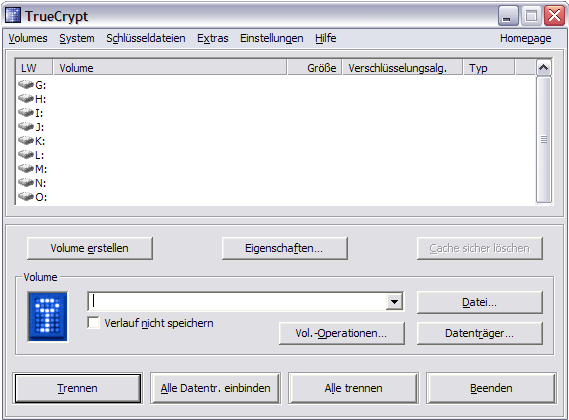
\includegraphics[scale=0.5]{../screenshots/truecypt.png}
\caption{Hauptfenster von Truecrypt}
\label{abb:truecrypt_haupt}
\end{center}
\end{figure}

\subsection{Verschl�sselten Container �ffnen}
Truecrypt-Container werden beim �ffnen grunds�tzlich als neue Laufwerke eingeh�ngt.
Das in Bild \ref{abb:truecrypt_haupt} dargestellte Hauptfenster von Truecrypt bietet die M�glichkeit, einen Buchstaben f�r das Laufwerk und die einzubindende Container-Datei bzw. den Datentr�ger zu w�hlen.\\

Zu beachten ist die Option \textit{Verlauf nicht speichern}. Ist diese Option aktiv, wird die Historie der ge�ffneten Container st�ndig gel�scht. Die Container sind auf der Festplatte oder dem USB-Stick nicht anhand eines speziellen Header als verschl�sselte Bereiche erkennbar. Sie sehen aus, wie zuf�lliger Datenm�ll.\\

\begin{figure}[htb]
\begin{center}
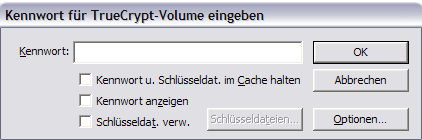
\includegraphics[scale=0.5]{../screenshots/truecrypt_use1.png}
\caption{Eingabe des Schl�ssels}
\label{abb:truecrypt_open}
\end{center}
\end{figure}

Anschlie�end ist der Button \textit{Einbinden} zu w�hlen. Das in Bild \ref{abb:truecrypt_open} dargestellte Fenster zur Eingabe der Schl�ssel erscheint. Hier ist der Schl�ssel f�r das �ffnen des Containers einzugeben (die Passphrase oder/und das Keyfile).\\

Einige Abk�rzungen f�r das �ffnen von Containern:
\begin{itemize}
 \item Ein Klick auf eine Datei mit der Endung .tc im Explorer �ffnet das Hauptfenster von Truecrypt und setzt den Namen der Datei als zu �ffnendes Volume.
\item Es ist m�glich, Favoriten zu definieren und diese alle zusammen �ber den Men�punkt \textit{Volumes -> Favoriten einbinden} einzubinden. Favoriten definiert man, indem diese Container eingebunden werden und anschlie�end die Konfiguration �ber den Men�punkt \textit{Volumes -> als Favoriten speichern} gesichert wird.
\item Als Favoriten definierte Container k�nnen bei Start von Truecrypt automatisch eingebunden werden. Unter \textit{Einstellungen -> Voreinstellungen} ist hierf�r die entsprechende Option zu aktivieren.
\item Wird Truecrypt bei der Anmeldung automatisch gestartet, k�nnen auch die Favoriten bei Anmeldung eingebunden werden.
\item Der Button \textit{Alle Datentr. einbinden} untersucht alle Partitionen und USB-Sticks auf Verschl�sselung. Es erscheint nacheinander der Dialog f�r die Schl�sseleingabe. Der Vorgang kann einige Zeit dauern.
\end{itemize}

\subsection{Verschl�sselten Container schlie�en}
Alle ge�ffneten Container werden standardm��ig bei der Abmeldung geschlossen. Au�erdem gibt es mehrere M�glichkeiten, einen ge�ffneten Container w�hrend der Arbeit wieder zu schlie�en:
\begin{itemize}
 \item Ein Klick mit der rechten Maustaste auf das Truecrypt-Icon im Systray �ffnet ein Men�, welches f�r alle eingebundenen Container das Trennen anbietet.
\item Im Hauptfenster von Truecrypt kann man mit der rechten Maustaste auf einen eingebundenen Container klicken und ihn trennen.
\item Der Button \textit{Alle trennen} im Hauptfenster von Truecrypt schlie�t alle eingebundenen Container.
\end{itemize}

ACHTUNG: Auch ein Beenden von Truecrypt im Systray schlie�t die Container nicht(!). Der D�mon l�uft weiter. Erst die Abmeldung des Nutzers oder ein Ausschalten des Systems schlie�t alle Container.

\subsection{WINDOWS komplett verschl�sseln}
Die aktuelle Version von Truecrypt erm�glicht es, WINDOWS bei laufenden Betrieb in einen verschl�sselten Container zu verschieben. Damit ist es f�r einen heimlichen Besucher sehr schwer, das System im ausgeschalteten Zustand zu kompromittieren. Es ist jedoch nicht unm�glich, wie das Stoned Bootkit zeigt, siehe \href{http://www.stoned-vienna.com/}{http://www.stoned-vienna.com}.\\

\textbf{Wichtig:} Vorrausetzung f�r die Nutzung dieses Features ist die M�glichkeit, ein CD-ISO-Image zu brennen. Dieses Image, welches w�hrend der Installation angelegt und gepr�ft wird, enth�lt wesentliche Daten f�r die Wiederherstellung, wenn es zu Bitfehlern im Header der Systempartition kommt.\\

\begin{figure}[htb]
\begin{center}
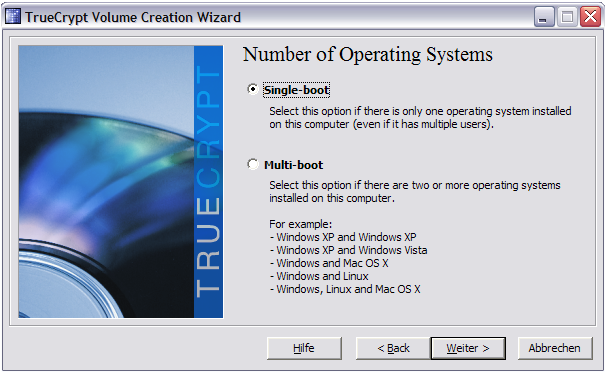
\includegraphics[scale=0.5]{../screenshots/truecrypt_sys_1.png}
\caption{Assistent f�r die System-Verschl�sselung}
\label{abb:truecrypt_sys}
\end{center}
\end{figure}

Den Assistent f�r die Systemverschl�sselung startet man im Hauptfenster von Truecrypt �ber den Men�punkt \textit{System - Encrypt System Partition}. Als Erstes wird abgefragt, ob nur die Partition von WINDOWS verschl�sselt werden soll oder die gesamte Festplatte. Die Verschl�sselung der gesamten Festplatte funktioniert nicht, wenn die Platte eine erweiterte Partition mit logischen Partitionen enth�lt oder wenn mehrere Betriebssysteme installiert sind.\\

Da der Masterboot-Record modifiziert wird, bem�ht sich Truecrypt, h�ufige Kombinationen verschiedener Betriebssysteme zu ber�cksichtigen.\\

Nach der Abfrage des Algorithmus f�r die Verschl�sselung, der Passphrase (Die mindestens 20 Zeichen lang sein sollte, Keyfiles k�nnen nicht genutzt werden!), und der Generierung von Zufallszahlen folgt die Erstellung der Rescue Disk (Bild \ref{abb:truecrypt_rescue}).\\

\begin{figure}[htb]
\begin{center}
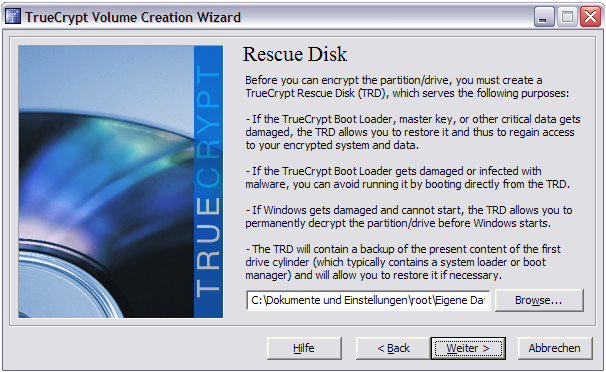
\includegraphics[scale=0.5]{../screenshots/truecrypt_sys_2.png}
\caption{Erstellung der Rescue-Disk}
\label{abb:truecrypt_rescue}
\end{center}
\end{figure}

Die Rescue-Disk wird als ISO-Image auf der Festplatte abgelegt und ist auf eine CD zu brennen. Die neue CD ist ins Laufwerk einzulegen. Truecrypt arbeitet erst weiter, wenn es die korrekte Erstellung der CD �berpr�ft hat.\\

Im vorletzten Schritt, stellt Truecrypt mehrere M�glichketen zum L�schen der alten, unverschl�sselten Daten zur Auswahl. Es gen�gt, die Daten einmal zu �berschreiben. Dabei werden nicht die einzelnen Dateien �berschrieben, sondern die Platte wird sektorenweise bearbeitet. Das garantiert, dass auch Fragmente gel�schter Dateien beseitigt werden.\\

Da es sich bei der Systemverschl�sselung um einen tiefen Eingriff handelt, f�hrt Truecrypt als n�chstes einen Test durch. Der PC wird neu gebootet und der Anwender muss am Bootloader sein Passwort eingeben.\\

Erst wenn dieser Test erfolgreich war, erfolgt die Verschl�sselung des Systems. Dieser Vorgang nimmt je nach Gr��e der Platte einige Zeit in Anspruch, ca 1-2min pro GByte.\\

Nach Abschlu� der Operation ist das System neu zu booten. Dabei wird vom Bootloader wieder das Passwort f�r den Zugriff auf die Systempartition abgefragt.

\subsection{Traveller Disk erstellen}
Truecrypt erm�glicht es, unter dem Men�punkt \textit{Extras -> Traveller Disk erstellen} einen USB-Stick zu verschl�sseln und zus�tzlich die Software selbst in einem unverschl�sselten Bereich hinzuzuf�gen.\\

Der Stick kann so konfiguriert werden, dass beim Anschlie�en des Sticks mit Hilfe der Autostart Funktion Truecrypt startet, den verschl�sselten Container einbindet und den Explorer �ffnet.\\

Dieses Feature soll es erm�glichen, einen verschl�sselten USB-Stick auch an Computern zu nutzen, auf denen Truecrypt nicht installiert ist.\\

Da man f�r diese Funktion Rechte als Administrator auf dem fremden Rechner ben�tigt, halte ich das Feature eher f�r Spielerei. Ein verantwortungsvoller Eigent�mer hat mir noch nie diese Rechte einger�umt und auch ich w�rde mir gut �berlegen, ob jemand auf meinem Rechner Software installieren darf. F�r viele Nutzer k�nnte es aber ein sinnvolles Feature sein.\\
% \section{TrueCrypt f�r Linux}
TrueCrypt, haupts�chlich f�r WINDOWS entwickelt, steht auch f�r Linux zum Download zur Verf�gung - eine Option f�r alle, die verschl�sselt Daten zwischen Linux und WINDOWS tauschen m�chten.\\

\textbf{Achtung:} Die Linux-Version verwendet ein eigenes Kernel-Modul f�r den Datenzugriff. Dieses ist nach einem Update des Kernels oder einem Upgrade der Distribition wahrscheinlich unbrauchbar. Die gesamte Installation muss erneut durchlaufen werden. Solange die verwendete Distribution kein zum Kernel passend kompiliertes TrueCrypt bietet, w�rde ich die Verwendung auf den Datenaustausch mit WINDOWS beschr�nken.\\

Mit \textbf{OneKript} steht auf Sourceforge.net ein grafisches GUI f�r Linux zum Download bereit. Dieses GUI ist f�r KDE konzipiert und nutzt den Kommander. \href{http://onekript.sourceforge.net/}{http://onekript.sourceforge.net/}

\subsubsection*{Installation}
Die komplexe Installation ist von en Entwicklern gut gel�st. Man ben�tigt die Quellen des verwendeten Kernel, welche mit den Tools zur Packetverwaltung installiert werden k�nnen.\\

Das TrueCrypt-Archiv ist nach dem Download in das Verzeichnis \textit{/usr/src} zu entpacken. Anschlie�end ist in das Verzeichnis mit den Linux-Sourcen zu wechseln und die �bersetzung mit em Script \textit{build.sh} zu starten. Das Ergebnis wird dann mit \textit{install.sh} installiert.

\begin{verbatim}
  # tar -xzf truecrypt-4.2.a-source-code.tgz -C /usr/src
  # cd /usr/src/truecrypt-4.2.a/Linux
  # ./build.sh
  .....
  # ./install.sh
\end{verbatim}

Die �bersetzung dauerte auf meinem Rechner mehr als 30min. Anscheinend wird dabei auch der Kernel neu kompiliert (aber nicht installiert!).

\subsubsection*{Container �ffnen}
F�r den transparenten Zugriff auf verschl�sselte Container wird der Device-Mapper genutzt. Das �ffnen eines Containers erfolgt in zwei Schritten:
\begin{enumerate}
 \item Als erstes wird der Container dem Device-Mapper unterstellt. Im Beispiel wird die verschl�sselte Containerdatei \textit{geheim.tc} vom USB-Stick als erstes TrueCrypt Device gemappt.
\begin{verbatim}
  > truecrypt -N 1 /media/usbstick/geheim.tc
\end{verbatim}
\item Anschlie�end kann das Device mit dem mount-Befehl in das Dateisystem eingebunden werden, beispielsweise nach \textit{/mnt}.
\begin{verbatim}
   > mount /dev/mapper/truecrypt1 /mnt
\end{verbatim}
\end{enumerate}

Beide Schritte k�nnen mit dem folgenden Kommando zusammengefasst werden, welches automatisch das n�chste freie TrueCrypt Device nutzt.
\begin{verbatim}
  > truecrypt /media/usbstick/geheim.tc /mnt
\end{verbatim}

\subsubsection*{Container schlie�en}
Auch das Schlie�en eines Containers erfolgt in zwei Schritten. Als estes ist das Device mit dem umount-Befehl auszuh�ngen, anschlie�end wird das Mapping des Containers aufgehoben:
\begin{verbatim}
  > umount /mnt
  > truecrypt -d 1
\end{verbatim}

Auch hier gibt es ein Vereinfachung. Das folgende Kommando h�ngte alle TrueCrypt Devices aus und schlie�t die Container:
\begin{verbatim}
  > truecrypt -d
\end{verbatim}

\subsubsection*{Weitere Features}
Es ist auch unter Linux m�glich, versch�sselte Container zu erstellen. Der folgende Befehl startet die Erstellung einer verschl�sselten Containerdatei auf dem USB-Stick. Dabei werden alle Informationen nacheinander abgefragt:
\begin{verbatim}
  > truecrypt -c /media/usbstick/geheim.tc
\end{verbatim}

Da TrueCrypt sehr empfindlich auf Bitfehler im Kopf der Datei reagiert, empfehlen die Entwickler, eine Sicherung des Headers zu speichern um diesen bei Bedarf wieder herstellen zu k�nnen:
\begin{verbatim}
  > truecrypt --backup-header BackupDatei Container
\end{verbatim}

Mit dem folgenden Befehl kann ein gesicherter Header wieder hergestellt werden:
\begin{verbatim}
  > truecrypt --restore-header BackupDatei Container
\end{verbatim}

\end{document}